\section{Numerical Optimizations}

\subsection{Bit-Parallel Monte Carlo}

\begin{figure}
\centering
\begin{tabular}{cccc}
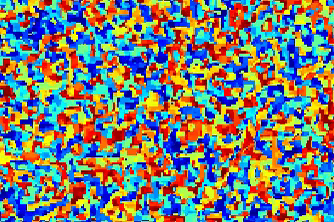
\includegraphics[height=.75in, trim={.7cm 0 .7cm 0},clip]{Parallel_Bits/iso-01}&
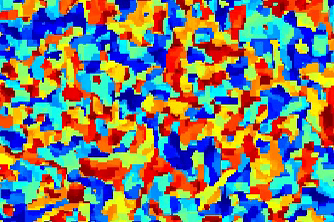
\includegraphics[height=.75in, trim={.7cm 0 .7cm 0},clip]{Parallel_Bits/iso-02}&
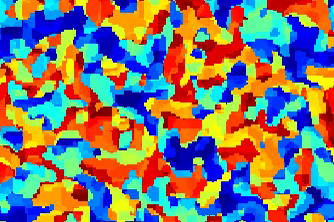
\includegraphics[height=.75in, trim={.7cm 0 .7cm 0},clip]{Parallel_Bits/iso-03}&
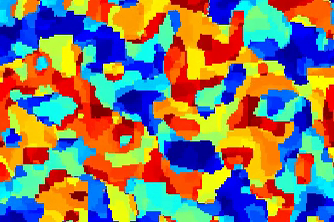
\includegraphics[height=.75in, trim={.7cm 0 .7cm 0},clip]{Parallel_Bits/iso-04}\\
%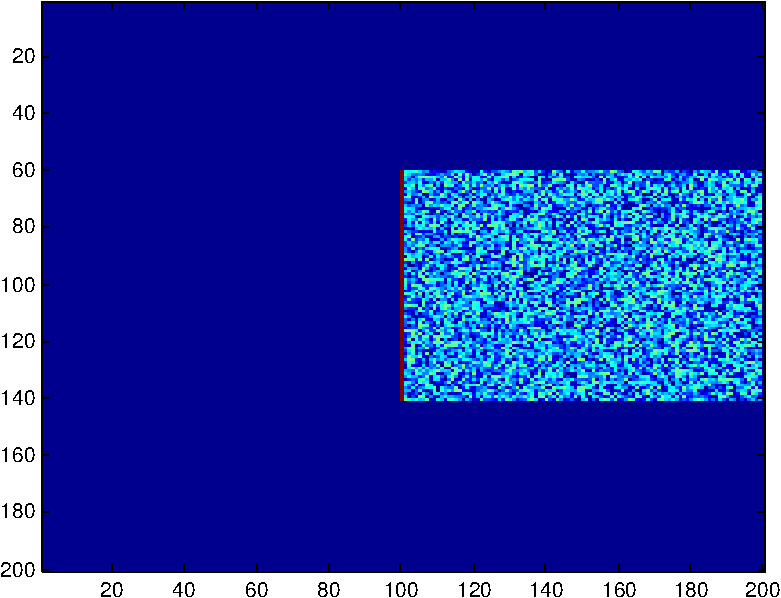
\includegraphics[height=.5in]{Parallel_Bits/par000}
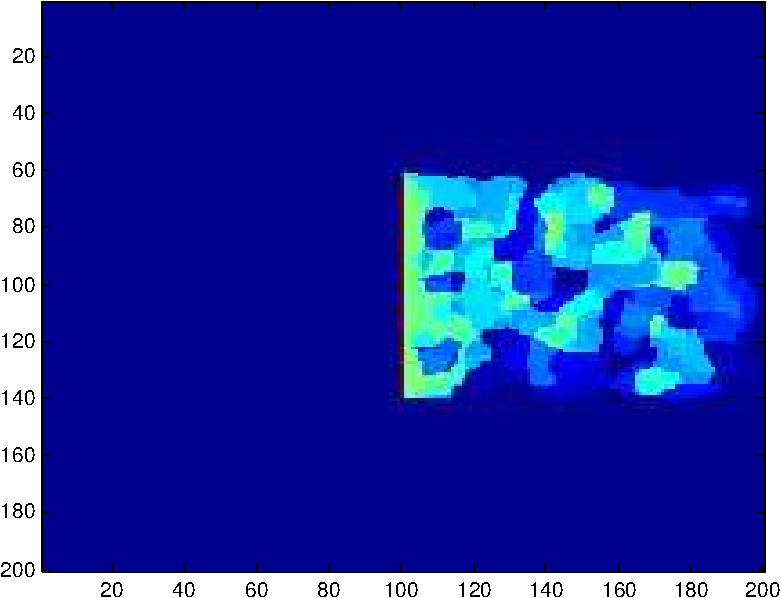
\includegraphics[height=.75in, trim={.7cm .6cm .7cm .6cm}, clip]{Parallel_Bits/par025}&
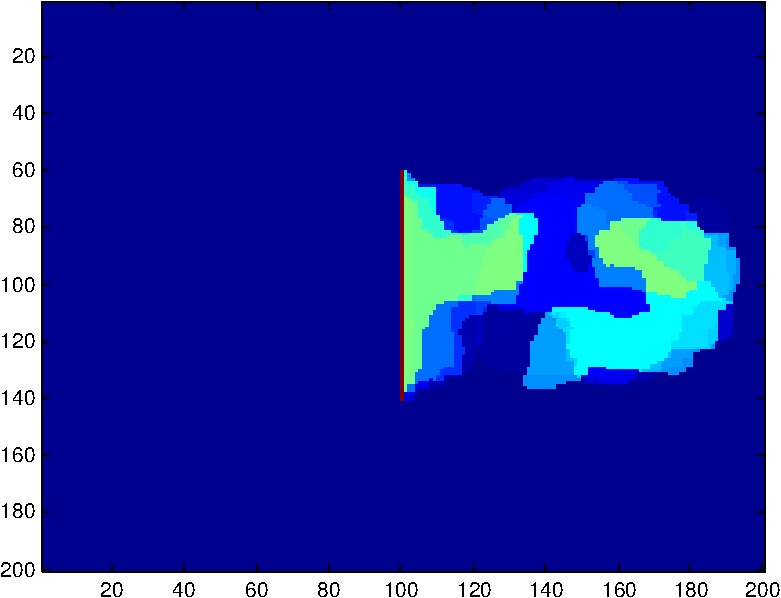
\includegraphics[height=.75in, trim={.7cm .6cm .7cm .6cm}, clip]{Parallel_Bits/par100}&
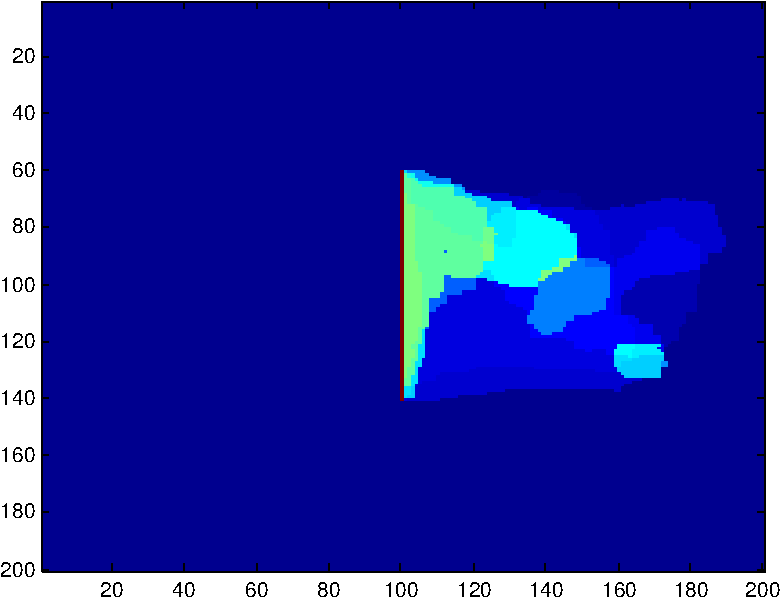
\includegraphics[height=.75in, trim={.7cm .6cm .7cm .6cm}, clip]{Parallel_Bits/par225}&
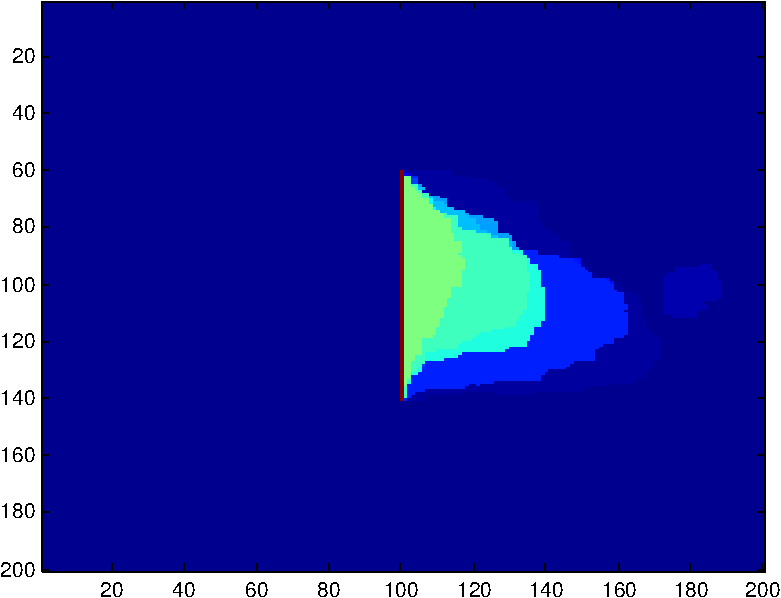
\includegraphics[height=.75in, trim={.7cm .6cm .7cm .6cm}, clip]{Parallel_Bits/par400}
\end{tabular}
\caption{\emph{Bit-Parallel Computation of Ising Marginal}
``Bit twiddling'' allows us to compute 64 simultaneous realizations of the Ising process
on a single array of long integers.  In the plots above, color is assigned according
to nominal integer value,
i.e.\, each realization contributes according to the significance of its bit position.
This is the most direct way of visualizing the data, and the exponential decay of bit
significance gives a sense of transparency and depth. Cf. Fig. \ref{fig: ising}
}
\end{figure}

Recall that the update probability for our Monte Carlo Ising process is
\def\bI{\bar{I}}
\def\ber{\operatorname{Bernoulli}}
\begin{align}
P(I^{t+1}_{ij} = 1|I^t) = \frac{\exp\bigl(\beta (H_{ij}^t-2)\bigr)}
{\exp\bigl(\beta (H_{ij}^t-2) \bigr) + \exp\bigl(-\beta (H_{ij}^t-2) \bigr)}
\end{align}
where
$$H_{ij}^t := I^t_{i+1,j} + I^t_{i,j+1} + I^t_{i-1,j} + I^t_{i,j-1}$$
This computation, which produces a single random bit, requires a new random floating-point number to be generated each time it is run.  
Many such bits need to be averaged to compute the marginal obstacle probabilities.
If this operation could be approximated using only bit-wise operations, we could run these operations in parallel, one for each
bit in a multi-bit datatype.  
%\dundundrvyion{O
\subsubsection{Overview}
We define a random process $\bI_{ij}^t$ to approximate $I_{ij}^t$.  For simplicity,
$\bI$ will take values in $\{0,1\}$, where $I$ took values in $\{-1,1\}$.
First, we generate a random bit $B \sim \ber(0.5)$. Recursively define
\begin{equation}
B^0 := B,\qtx{and}B^k := B^{k-1}_1\wedge B^{k-1}_2 ,
\end{equation}
where $B^{k-1}_{1,2} \sim B^{k-1}$ are i.i.d.\ copies (their generation is discussed in the next section).
Thus $B^k \sim \ber(2^{-2^k})$.
Define
\begin{equation}
 \bI^{t+1}_{ij} := \begin{cases}
B(\bar H_{ij}^t) & \bar H_{ij}^t<2\\
\neg B(\bar H_{ij}^t) & \bar H_{ij}^t>2\\
B^0 & \bar H_{ij}^t=2
\end{cases},
\end{equation}
where
\begin{gather}
B(H) := \bigwedge_{k=1}^K((\neg C_k(H))\vee B^k),\\
C_k(H) := \text{$k$-th bit of}\; \bar{\beta}|H-2|+1.
\end{gather}
Here $\bar\beta$ must be an integer. Observe that 
$$\exp_2\bigl(-\sum_{k=1}^K 2^k\,C_k(H)\bigr) =  2^{-\bar\beta |H-2|-1},$$
and thus
\begin{equation}
E(\bI^{t+1}_{ij}) = 
\begin{cases}
2^{-\bar\beta |H-2|-1} & H_{ij}^t < 2\\
1-2^{-\bar\beta |H-2|-1} & H_{ij}^t > 2\\
0.5 & H_{ij}^t = 2
\end{cases}
\end{equation}

\begin{figure}
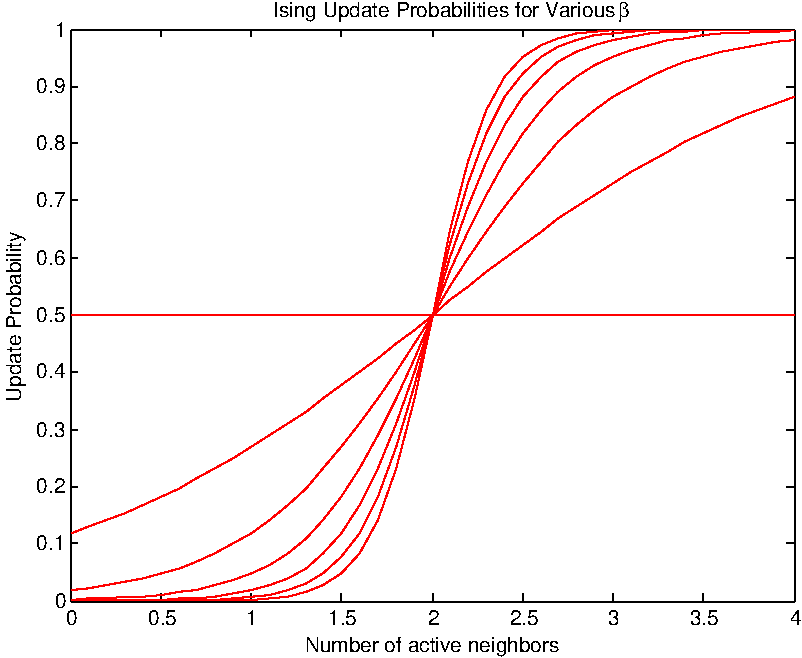
\includegraphics[width=1.5in]{Parallel_Bits/isingup}\quad
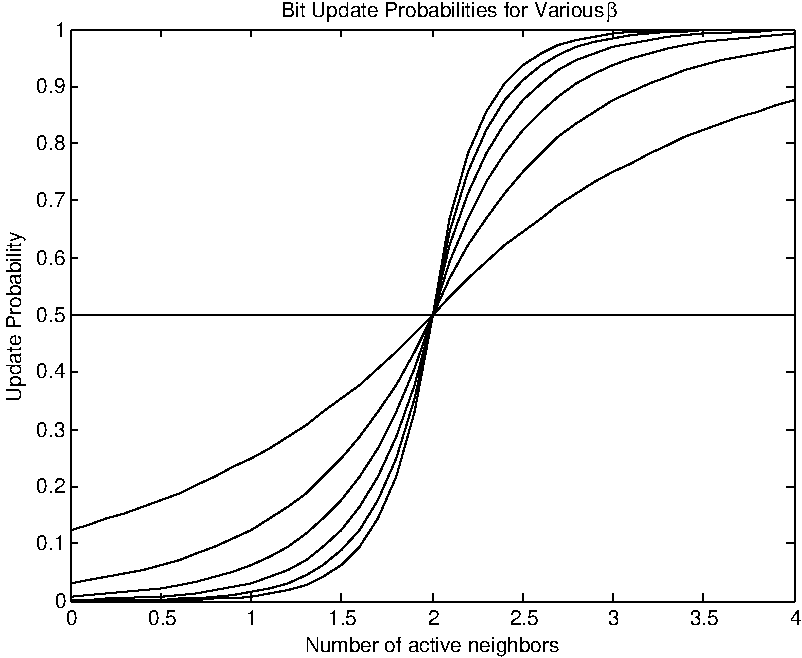
\includegraphics[width=1.5in]{Parallel_Bits/bitup}\quad
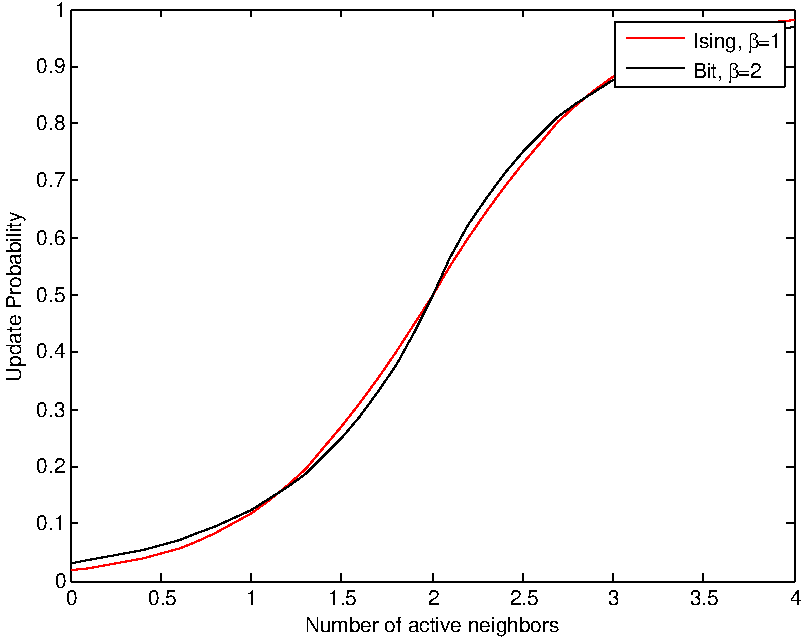
\includegraphics[width=1.5in]{Parallel_Bits/parcompare}
\caption{\emph{Comparison of Update Probabilities:} 
Values of $\bar\beta$ are taken from 0 to 6.  
Update probabilities for the Ising Model and
the parallel bit estimate are computed on the continuum $[0,4]$, 
although only integers $\{0, \ldots 4\}$ are used in practice.\label{fig: parcompare}}
\end{figure}
\subsubsection{Computing the counts $C_k$}

The counting bits $C_k$ are computed as with a standard binary adder.  
This requires $O(k)$ bitwise AND and/or XOR operations for binary sum and carry,
and about $2k$ boolean variables as registers.

\subsubsection{Generating I.I.D. Bits}

equivalent to the conjunction of $2^k$ independent coin-flips $B_i^0$:
$$B^k \sim B^0_1 \wedge B^0_2 \wedge \cdots B^0_{2^k}.$$
Instead of calling the random number generator $2^k$ times,
we generate a single $N$-bit ($N\geq2^k$) integer $L$ (for ``long''), and 
conjoin it with $k$ bit-shifted copies of itself.  Recursively define
\begin{equation}
L^0 := L, \qquad L^k := (L^{k-1} \wedge (L^{k-1} \ll 2^{k-1})) \ll 3\cdot 2^{k-1}-2.
\end{equation}
Observe that
\begin{align*}
L^k &= (L^{k-1} \wedge (L^{k-1} \ll 2^{k-1})) \ll 3\cdot 2^{k-1}-2 \\
&= (L^{k-1} \ll 2^{k-1}) \wedge (L^{k-1} \ll 2\cdot 2^{k-1}) \ll 2^k-2 \\
&= (L^{k-1} \ll 2^{k-2}) \wedge (L^{k-2} \ll 2\cdot 2^{k-2})\\
&\qquad\wedge (L^{k-1} \ll 3\cdot2^{k-2}) \wedge (L^{k-2} \ll 4\cdot 2^{k-2})  \ll 2^k-2\\ 
&\quad\vdots\\
&= \Bigl(\bigwedge\nolimits_{j=0}^{\!\!2^k-1} \bigl(L^0 \ll j\bigr)\Bigr) \ll 2^k-1.
\end{align*}
Thus, for the $i$-th bit of $L^k$:
\def\ww{\,\wedge\,}
\begin{align*}
(L^k)_i %&= (L^{k-1})_{i-2^{k-1}} \ww (L^{k-1})_{i-2\cdot2^{k-1}}\\
%&= (L^{k-2})_{i-2^{k-2}} \ww (L^{k-2})_{i-2\cdot2^{k-2}} \ww (L^{k-2})_{i-3\cdot2^{k-2}} \ww (L^{k-2})_{i-4\cdot2^{k-2}} \\
%&\quad\vdots\\
&= \bigwedge\nolimits_{j=2^k-1}^{\!\!2^{k+1}-2} L^0_{i-j}
\end{align*}
where bit indices are taken modulo $N$.  
This is a $2^k$-fold conjunction of independent random bits, so 
$$P((L^k)_i=1) = 2^{-2^k},$$
Observe, also, that the bits 
$$(L^{k_1})_i = \bigwedge\nolimits_{j=2^k-1}^{\!\!2^{k+1}-2} L^0_{i-j} \qtx{and}
(L^{k_2})_i = \bigwedge\nolimits_{j=2^k-1}^{\!\!2^{k+1}-2} L^0_{i-j}$$
are independent for $k_1\neq k_2$ (the ranges $[2^{k_1}-1, 2^{k_1+1}-2]$
and $[2^{k_2}-1, 2^{k_2+1}-2]$ do not overlap).
Note, however that when indices $i_1$ and $i_2$ differ by less than $2^k$,
the bits $(L^k)_{i_1}$ and $(L^k)_{i_1}$ are highly correlated, especially for large $k$.

In modern processors, the bit-shift operation runs in constant time, so
the random lookup integers $\{L^k, \ldots, L^k\}$ are generated in $O(K)$ time.

\iffalse
\subsection{Mesh}
\begin{figure}
\begin{tabular}{ccc}
\centering
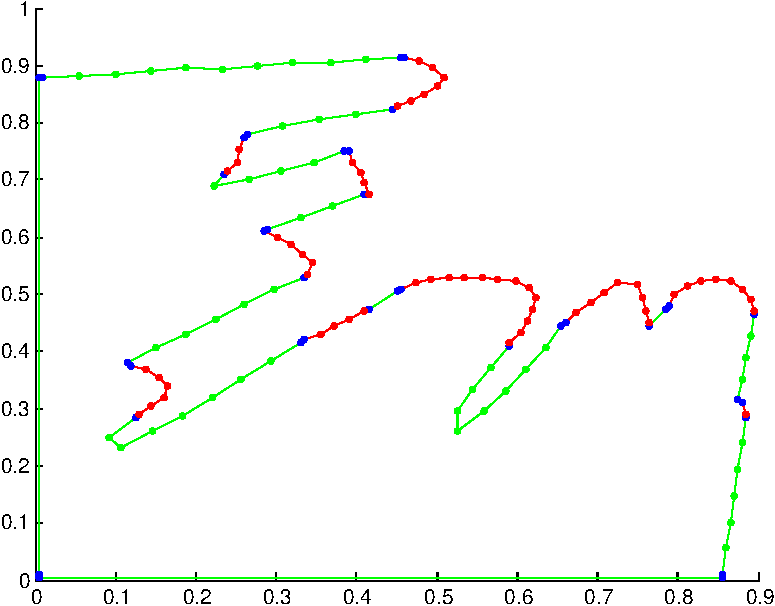
\includegraphics[height=1.2in]{mesh/Boundaries}&
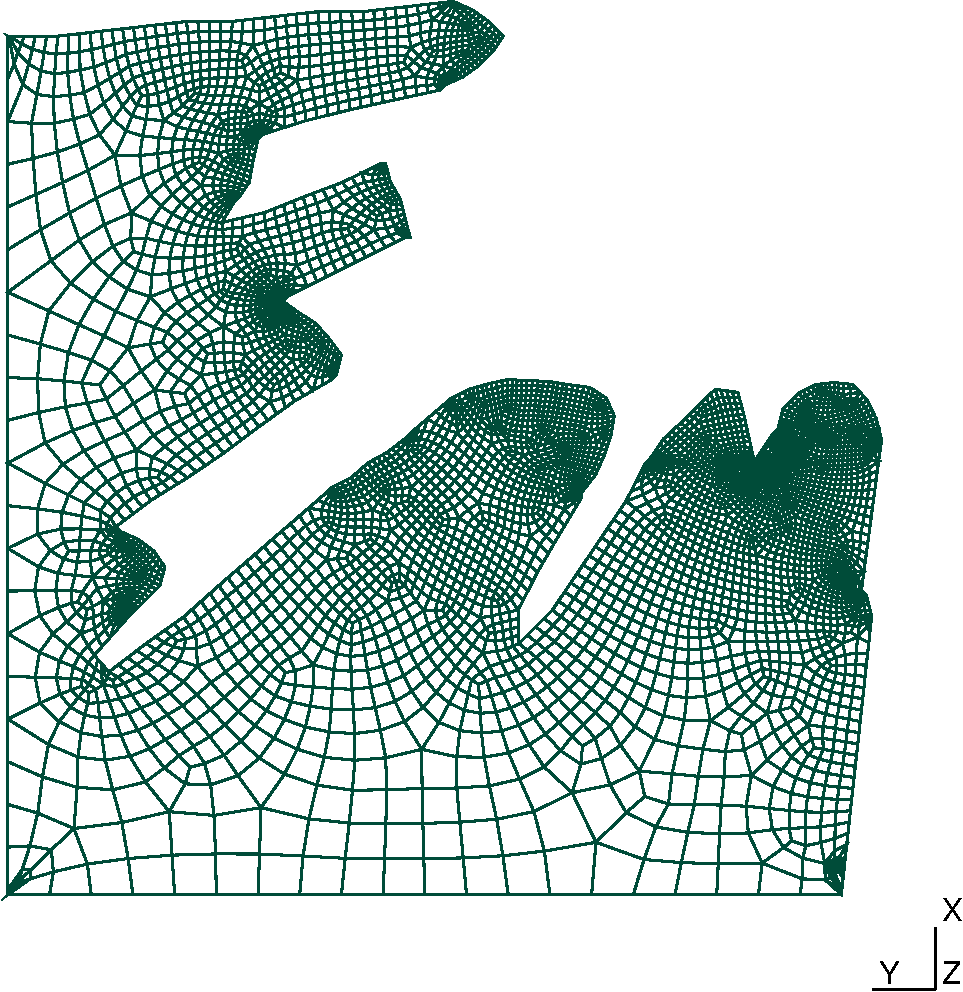
\includegraphics[height=1.2in]{mesh/mesh}&
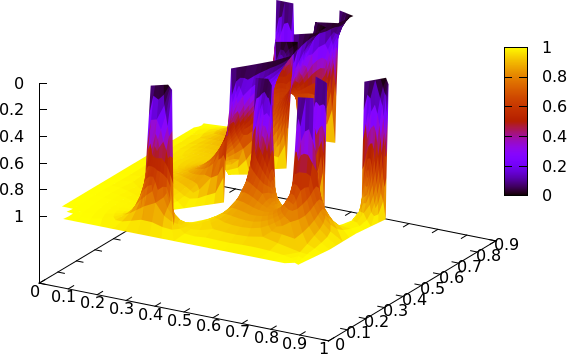
\includegraphics[height=1.2in]{mesh/solution}
\end{tabular}
\caption{\emph{Finite-Element Approximation}}
\end{figure}
\fi